\documentclass[conference]{IEEEtran}

\usepackage{graphicx}
\usepackage{booktabs}
\usepackage{amsmath}
\usepackage{amssymb}
\usepackage{cite}
\usepackage[hidelinks]{hyperref}

\providecommand{\tightlist}{%
  \setlength{\itemsep}{0pt}%
  \setlength{\parskip}{0pt}%
}

\title{
Residual-Risk-Guided Discovery of
Stochastic Mixed-Order Capability Interactions
}

\author{
\IEEEauthorblockN{Anonymous Author(s)}
\IEEEauthorblockA{Anonymous Submission}
}

\begin{document}

\maketitle

\begin{abstract}
Modern AI systems combine capabilities such as tool use, structured output, streaming, reasoning, and multimodal processing. Failures may emerge only from particular capability combinations, creating stochastic interaction bugs that are difficult to isolate through independent testing. Exhaustive combinatorial discovery can identify such interactions but becomes increasingly expensive as capability count and interaction order grow.

We present SCIF v0.0.4, a residual-risk-guided method for stochastic mixed-order interaction discovery. SCIF first screens and confirms pairwise interactions, suppresses those already supported by the data, measures the remaining empirical failure risk, and invokes higher-order localization only when substantial unexplained risk remains.

Evaluation on the synthetic BSIB benchmark family produced 6,999 exact recoveries across 7,000 unseen holdout runs (99.9857\%), with no observed false interaction candidates. In a 100-seed method comparison, SCIF V4 recovered all evaluated pairwise, overlapping, pure-three-way, and mixed-order structures; pairwise SCIF and deletion localization both achieved 0\% exact recovery on the mixed scenario. For that eight-capability benchmark, SCIF required 22,800 mean simulator executions versus 93,000 for exhaustive order-three discovery, a 75.48\% reduction.

Ablation experiments confirmed distinct roles for residual-risk detection and higher-order localization. Across scaling experiments from eight to twenty capabilities, SCIF achieved 20/20 observed exact recoveries at each size while execution reduction reached 96.14\%. These results support residual-risk-guided escalation as a promising approach for stochastic interaction discovery, while external validation beyond synthetic benchmarks remains future work.

\end{abstract}

\input{generated/00_introduction.tex}

\input{generated/01a_related_work.tex}

\section{Research Questions}

This study evaluates whether residual-risk-guided escalation can recover stochastic mixed-order capability interactions accurately while reducing the cost of exhaustive higher-order discovery.

\subsection{RQ1 --- Discovery Accuracy}

\textbf{How accurately does SCIF v0.0.4 recover hidden interaction structures under stochastic outcomes?}

We evaluate exact recovery, missed interactions, and observed false interaction candidates across the unseen BSIB holdout.

\subsection{RQ2 --- Efficiency Relative to Baselines}

\textbf{How does SCIF v0.0.4 compare with pairwise discovery, deletion localization, and exhaustive discovery?}

We compare both exact interaction recovery and simulator execution cost on representative pairwise, overlapping, pure-three-way, and mixed-order scenarios.

\subsection{RQ3 --- Contribution of Residual-Risk Reasoning}

\textbf{Do residual-risk detection and higher-order localization provide distinct benefits?}

Ablation experiments compare pairwise discovery alone, pairwise discovery with residual-risk detection, and the complete SCIF V4 pipeline.

\subsection{RQ4 --- Parameter Sensitivity}

\textbf{How sensitive is recovery to key sampling and localization thresholds?}

We vary initial sampling, residual-risk, and removal thresholds while monitoring recovery and false interaction candidates.

\subsection{RQ5 --- Scaling Behavior}

\textbf{How does SCIF behave as capability count increases?}

We measure exact recovery, simulator executions, reduction relative to exhaustive order-three discovery, and wall-clock behavior from 8 to 20 capabilities.


\section{Methodology}

\subsection{Problem Formulation}

Let

\[
K = \{k_1, k_2, \ldots, k_n\}
\]

denote the set of capabilities available to a system.

A capability configuration is a subset

\[
C \subseteq K.
\]

Executing configuration \(C\) produces a stochastic binary outcome

\[
Y(C) \in \{0,1\},
\]

where \(Y(C)=1\) denotes a failure.

Each configuration therefore has an unknown failure probability

\[
p(C)=P(Y(C)=1).
\]

The discovery problem is to identify minimal subsets of capabilities whose joint activation causes a substantial increase in failure risk, while minimizing the total number of stochastic executions required.

\subsection{Stochastic Capability Interactions}

A capability interaction is not defined only by a high absolute failure probability.

A candidate set must also exhibit risk beyond that observed in its relevant lower-order subsets.

For a candidate interaction \(C\), SCIF uses a joint-risk increment concept of the form

\[
JRI(C)
=
\hat{p}(C)
-
\max_{S \subset C}
\hat{p}(S),
\]

where \(\hat{p}\) denotes an empirical failure-rate estimate.

A candidate is therefore supported when its joint failure rate is sufficiently large and its observed risk cannot be explained by a lower-order subset.

\subsection{BSIB Benchmark Model}

The Benchmark for Stochastic Interaction Bugs (BSIB) provides synthetic capability configurations with hidden interaction faults.

The simulator exposes only stochastic execution outcomes to the discovery algorithm.

The underlying true failure probability is not included in the execution result.

This prevents the discovery algorithm from directly accessing the benchmark ground truth.

\subsection{Keyed Stochastic Simulation}

Experiments use deterministic keyed random streams.

For a fixed benchmark configuration and experiment seed, the random outcome stream is stable even when configurations are evaluated in a different order.

This design prevents algorithmic execution order from unintentionally changing the stochastic evidence observed for the same configuration.

The keyed simulator therefore supports reproducible and fair comparisons among discovery methods.

\subsection{Pairwise Discovery}

SCIF v0.0.4 begins with the SCIF v0.0.3 pairwise discovery procedure.

The frozen evaluation configuration uses:

\begin{itemize}
\tightlist
\item
  100 initial screening trials;
\item
  300 screening-retest trials;
\item
  1,500 confirmation trials;
\item
  1,000 subset-confirmation trials;
\item
  minimum joint failure rate of 0.15;
\item
  minimum joint-risk increment of 0.10; and
\item
  confidence threshold of 0.95.
\end{itemize}

Initial sampling provides a low-cost estimate of the failure signal.

Pairs with sufficiently convincing evidence proceed to confirmation.

Borderline configurations may receive additional screening trials before a final decision is made.

This architecture concentrates stochastic executions on configurations that show evidence of interaction risk.

\subsection{Limitation of Pairwise-Only Discovery}

A pure higher-order interaction can remain invisible to every lower-order subset.

For example, consider a three-way interaction involving capabilities

\[
\{a,b,c\}.
\]

It is possible for

\[
p(\{a,b\}),
p(\{a,c\}),
p(\{b,c\})
\]

to remain near baseline while

\[
p(\{a,b,c\})
\]

is substantially elevated.

A pairwise-only algorithm therefore cannot represent or recover this type of fault.

This limitation motivates the higher-order stages of SCIF v0.0.4.

\subsection{Known-Pair Suppression}

After pairwise discovery, SCIF v0.0.4 constructs probe configurations intended to disable already-discovered pairwise interactions.

For the set of discovered pairwise interactions, the algorithm computes minimal capability-removal sets that intersect every known pair.

Removing such a set creates a configuration in which the discovered pairwise interactions are suppressed.

Multiple minimal removal sets may exist.

SCIF evaluates the resulting residual configurations rather than assuming that one particular suppression is sufficient.

\subsection{Residual-Risk Detection}

Let \(C_r\) denote a configuration after suppression of known pairwise interactions.

SCIF estimates

\[
\hat{p}(C_r)
\]

and compares the remaining failure signal with the estimated baseline.

Higher-order escalation is triggered only when residual failure risk remains sufficiently large.

The frozen parameters are:

\begin{itemize}
\tightlist
\item
  1,000 residual trials;
\item
  minimum residual failure rate of 0.15; and
\item
  minimum residual-risk increment of 0.10.
\end{itemize}

Conceptually, the residual stage asks:

\begin{quote}
After explaining and suppressing the interactions already found, does substantial unexplained risk remain?
\end{quote}

If the answer is no, SCIF terminates without invoking higher-order localization.

If the answer is yes, the residual configuration becomes the input to the higher-order localizer.

\subsection{Residual Higher-Order Localization}

Higher-order localization is applied only after residual-risk detection has justified escalation.

For each capability in the selected residual configuration, SCIF measures the failure rate after removing that capability.

Let \(C_r\) be the source configuration and let \(k \in C_r\).

The empirical removal drop is

\[
D(k)
=
\hat{p}(C_r)
-
\hat{p}(C_r \setminus \{k\}).
\]

Capabilities whose removal causes a sufficiently large decrease in failure risk are treated as candidate members of the hidden interaction.

The frozen localization configuration uses:

\begin{itemize}
\tightlist
\item
  1,000 trials per configuration;
\item
  minimum failure rate of 0.15;
\item
  minimum removal drop of 0.10; and
\item
  minimum higher-order candidate size of three.
\end{itemize}

\subsection{Minimality Confirmation}

Removal evidence alone is not sufficient.

The resulting candidate is evaluated directly, and its immediate subsets are also tested.

The purpose is to verify that the candidate itself retains elevated failure risk while dropping one of its essential members removes the interaction signal.

This step protects against reporting unnecessarily large interaction sets.

\subsection{Complete SCIF v0.0.4 Pipeline}

The final procedure is:

\begin{enumerate}
\def\labelenumi{\arabic{enumi}.}
\tightlist
\item
  perform adaptive pairwise discovery;
\item
  record confirmed pairwise interactions;
\item
  construct minimal suppression sets for the known pairs;
\item
  evaluate residual-risk probes;
\item
  stop when no substantial residual risk remains;
\item
  otherwise select a residual configuration;
\item
  apply deletion-style higher-order localization;
\item
  confirm candidate minimality; and
\item
  return pairwise and higher-order discoveries in a unified report.
\end{enumerate}

The higher-order stage is therefore conditional rather than mandatory.

This design preserves the efficiency of pairwise discovery on simple scenarios while providing an escalation path for unexplained higher-order risk.


\section{Experimental Setup}

\subsection{Benchmark Scenarios}

The primary evaluation uses seven BSIB scenarios.

\subsubsection{NULL}

\texttt{BSIB-NULL-001} contains no hidden interaction.

It evaluates whether the method avoids reporting interactions when all configurations remain near baseline stochastic risk.

\subsubsection{PAIR-001}

\texttt{BSIB-PAIR-001} contains a strong pairwise interaction between:

\begin{itemize}
\tightlist
\item
  \texttt{tools}; and
\item
  \texttt{structured\_output}.
\end{itemize}

\subsubsection{PAIR-002}

\texttt{BSIB-PAIR-002} contains a weaker pairwise interaction between:

\begin{itemize}
\tightlist
\item
  \texttt{tools}; and
\item
  \texttt{streaming}.
\end{itemize}

This scenario is specifically useful for evaluating stochastic screening stability.

\subsubsection{PAIR-003}

\texttt{BSIB-PAIR-003} contains an interaction between:

\begin{itemize}
\tightlist
\item
  \texttt{parallel\_tools}; and
\item
  \texttt{strict\_schema}.
\end{itemize}

It serves as an additional unseen pairwise scenario.

\subsubsection{OVERLAP}

\texttt{BSIB-OVERLAP-001} contains two pairwise interactions that share one capability:

\begin{itemize}
\tightlist
\item
  \texttt{tools\ +\ streaming}; and
\item
  \texttt{streaming\ +\ strict\_schema}.
\end{itemize}

The scenario tests whether the discovery procedure can recover more than one overlapping pair.

\subsubsection{TRIPLE}

\texttt{BSIB-TRIPLE-001} contains the pure higher-order interaction:

\begin{itemize}
\tightlist
\item
  \texttt{tools\ +\ streaming\ +\ strict\_schema}.
\end{itemize}

Its proper pairs remain near baseline.

The scenario therefore provides no pairwise interaction signal for the hidden triple.

\subsubsection{MIXED}

\texttt{BSIB-MIXED-001} contains both:

\begin{itemize}
\tightlist
\item
  pair: \texttt{tools\ +\ streaming}; and
\item
  triple: \texttt{reasoning\ +\ strict\_schema\ +\ multimodal}.
\end{itemize}

The benchmark is designed to expose masking behavior that affects single-interaction deletion localization.

\subsection{Evaluation Metrics}

The principal metric is exact recovery.

A run is counted as exactly recovered only when the complete set of reported interactions equals the benchmark ground truth.

Additional measures include:

\begin{itemize}
\tightlist
\item
  pairwise recovery;
\item
  higher-order recovery;
\item
  residual-risk classification;
\item
  false-positive runs;
\item
  mean simulator executions;
\item
  median simulator executions;
\item
  minimum and maximum executions;
\item
  95th-percentile execution count;
\item
  reduction relative to exhaustive discovery; and
\item
  wall-clock time in the scaling experiment.
\end{itemize}

\subsection{Unseen Holdout Evaluation}

The primary holdout evaluation uses 1,000 unseen seeds per benchmark scenario.

The holdout seed range is:

\[
31001,\ldots,32000.
\]

Seven scenarios are evaluated, producing a total of

\[
7 \times 1000 = 7000
\]

SCIF v0.0.4 holdout runs.

Parameters were not modified after observing the holdout results.

This is important because one rare weak-pair miss was retained and analyzed rather than being used to retune the algorithm.

\subsection{Baseline Comparison}

Four discovery methods are compared:

\begin{enumerate}
\def\labelenumi{\arabic{enumi}.}
\tightlist
\item
  SCIF v0.0.3;
\item
  deletion-based localization;
\item
  exhaustive discovery; and
\item
  SCIF v0.0.4.
\end{enumerate}

The comparison study uses 100 seeds from:

\[
41001,\ldots,41100.
\]

The selected scenarios are:

\begin{itemize}
\tightlist
\item
  PAIR-002;
\item
  OVERLAP;
\item
  TRIPLE; and
\item
  MIXED.
\end{itemize}

For pairwise scenarios, exhaustive discovery evaluates configurations through order two.

For scenarios containing a triple, exhaustive discovery evaluates configurations through order three.

With eight capabilities this corresponds to:

\[
1 + 8 + \binom{8}{2}
=
37
\]

configurations for exhaustive order-two discovery, or 37,000 simulator executions at 1,000 trials per configuration.

For exhaustive order-three discovery:

\[
1 + 8 + \binom{8}{2} + \binom{8}{3}
=
93
\]

configurations are evaluated, corresponding to 93,000 simulator executions.

For adaptive methods, execution cost is the actual number of simulator invocations performed by the method, including screening, retesting, confirmation, residual probing, and localization where applicable. The exhaustive baselines instead use the fixed 1,000-trial budget for every enumerated configuration.

\subsection{Ablation Study}

The ablation study uses 100 seeds:

\[
51001,\ldots,51100.
\]

Five representative scenarios are evaluated:

\begin{itemize}
\tightlist
\item
  NULL;
\item
  PAIR-002;
\item
  OVERLAP;
\item
  TRIPLE; and
\item
  MIXED.
\end{itemize}

Three algorithmic stages are compared:

\subsubsection{Stage A --- V3 Pairwise Only}

Only confirmed pairwise discoveries are considered.

\subsubsection{Stage B --- V3 + Residual Detection}

Pairwise discovery is followed by residual-risk classification.

This stage determines whether higher-order escalation is needed but does not yet localize a higher-order interaction.

\subsubsection{Stage C --- Full V4}

The complete pipeline includes residual higher-order localization.

The ablation records:

\begin{itemize}
\tightlist
\item
  stage success;
\item
  false residual escalations;
\item
  missed escalations;
\item
  false higher-order candidates; and
\item
  mean execution cost.
\end{itemize}

\subsection{Sensitivity Study}

The sensitivity study uses 100 seeds:

\[
61001,\ldots,61100.
\]

Four scenarios are tested:

\begin{itemize}
\tightlist
\item
  NULL;
\item
  PAIR-002;
\item
  TRIPLE; and
\item
  MIXED.
\end{itemize}

The frozen baseline configuration is:

\begin{itemize}
\tightlist
\item
  \texttt{initial\_trials\ =\ 100};
\item
  \texttt{min\_residual\_increment\ =\ 0.10}; and
\item
  \texttt{higher\_order\_min\_removal\_drop\ =\ 0.10}.
\end{itemize}

The evaluated alternatives are:

\begin{itemize}
\tightlist
\item
  initial trials = 50;
\item
  initial trials = 200;
\item
  residual increment = 0.05;
\item
  residual increment = 0.15;
\item
  removal drop = 0.05; and
\item
  removal drop = 0.15.
\end{itemize}

The purpose is sensitivity characterization rather than post-holdout parameter optimization.

\subsection{Scaling Study}

Scaling is evaluated using benchmark variants with:

\begin{itemize}
\tightlist
\item
  8 capabilities;
\item
  12 capabilities;
\item
  16 capabilities; and
\item
  20 capabilities.
\end{itemize}

Each benchmark retains:

\begin{itemize}
\tightlist
\item
  one pairwise interaction; and
\item
  one three-way interaction.
\end{itemize}

Additional capabilities are non-interacting noise capabilities.

Twenty seeds are evaluated for each size:

\[
71001,\ldots,71020.
\]

For \(n\) capabilities, exhaustive order-three discovery evaluates

\[
1+n+\binom{n}{2}+\binom{n}{3}
\]

configurations.

At 1,000 trials per configuration, exhaustive execution counts are:

\begin{itemize}
\tightlist
\item
  93,000 for 8 capabilities;
\item
  299,000 for 12 capabilities;
\item
  697,000 for 16 capabilities; and
\item
  1,351,000 for 20 capabilities.
\end{itemize}

\subsection{Reproducibility}

The reproducibility package contains benchmark definitions, simulator implementation, discovery algorithms, automated tests, experiment scripts, aggregated result files, and publication figure-generation scripts.

All Python development commands are executed through a locked \texttt{uv} environment. Repository-identifying information is omitted during anonymous review.


\input{generated/04_results.tex}

\begin{figure}[t]
\centering
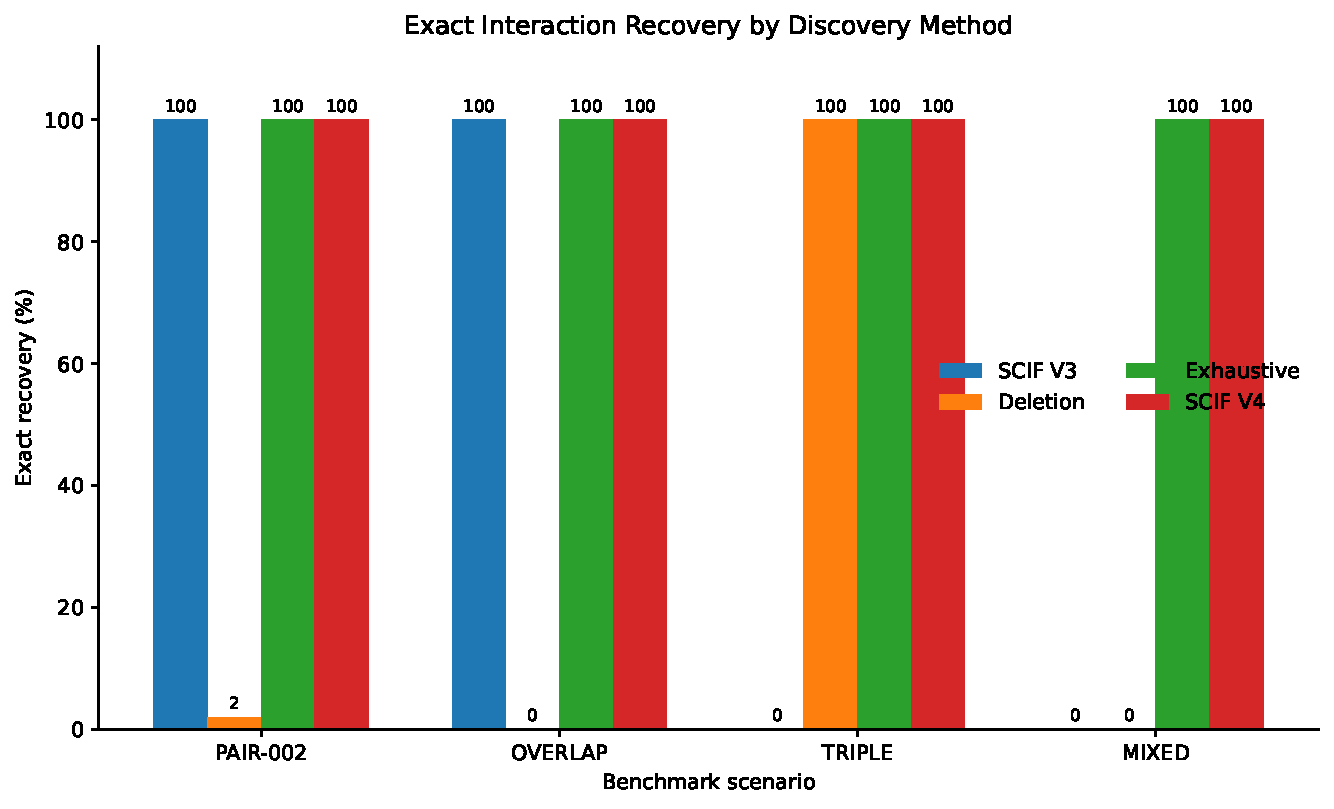
\includegraphics[
  width=0.94\columnwidth
]{figures/figure_1_recovery_comparison.pdf}
\caption{
Exact interaction recovery by discovery method.
}
\label{fig:recovery}
\end{figure}

\begin{figure}[t]
\centering
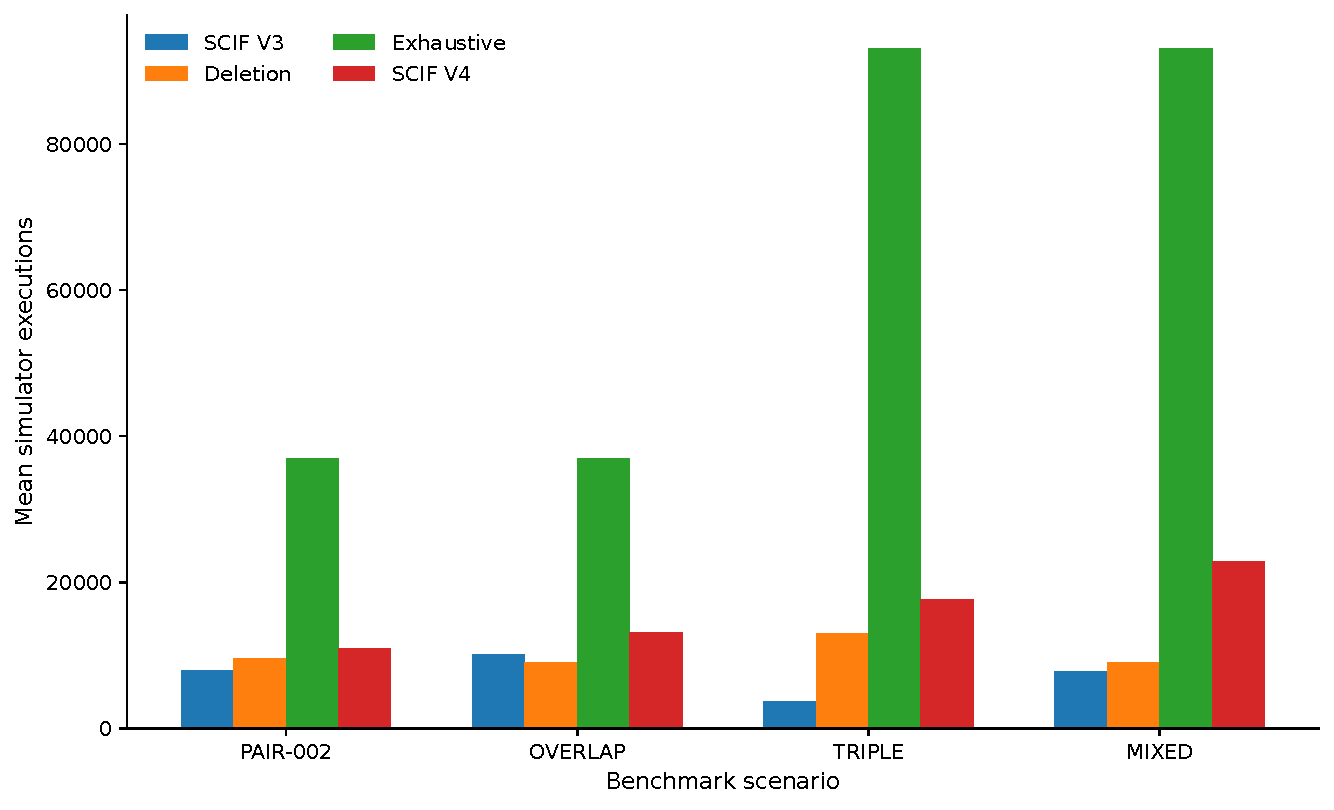
\includegraphics[
  width=0.94\columnwidth
]{figures/figure_2_execution_comparison.pdf}
\caption{
Mean simulator executions by discovery method.
}
\label{fig:executions}
\end{figure}

\begin{figure}[t]
\centering
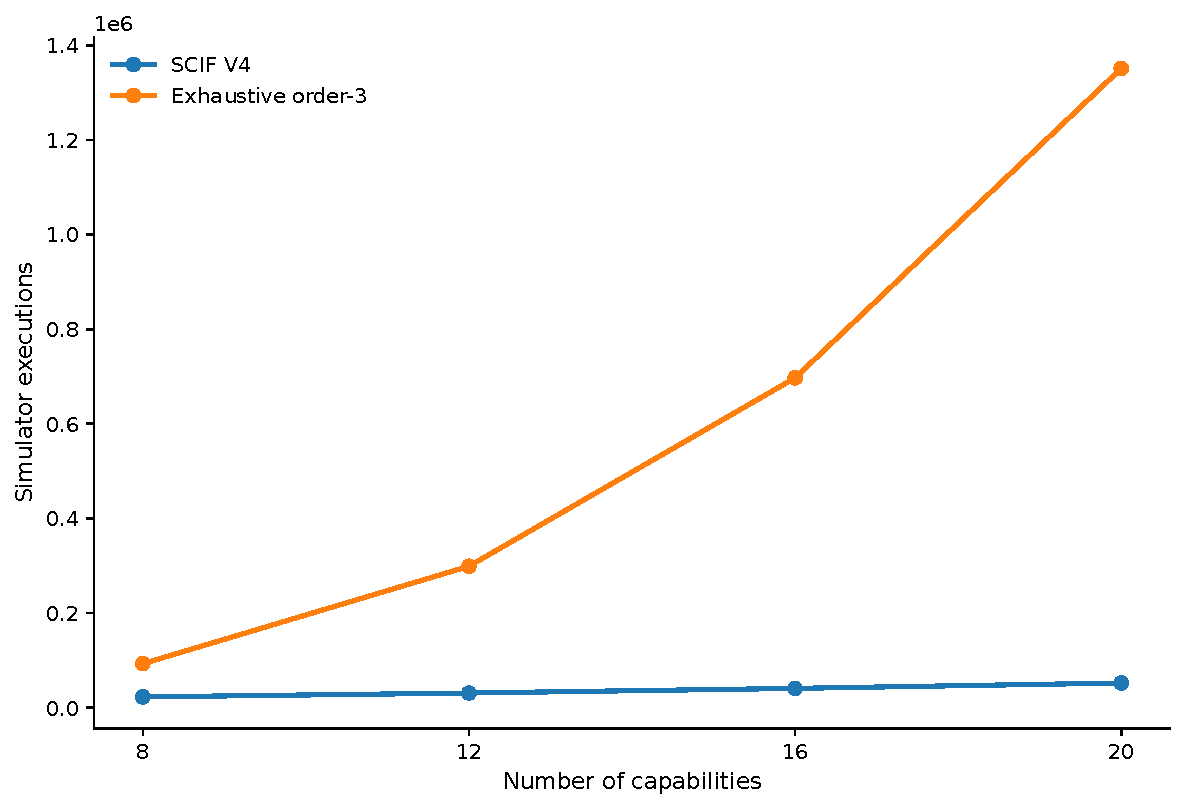
\includegraphics[
  width=0.94\columnwidth
]{figures/figure_3_scaling.pdf}
\caption{
Simulator execution scaling from 8 to 20 capabilities.
}
\label{fig:scaling}
\end{figure}

\section{Discussion}

\subsection{Main Interpretation}

SCIF's main advantage is the separation of already-explained risk from unexplained residual risk. Pairwise discovery handles interactions visible at order two, while higher-order localization is invoked only when risk remains after known pairwise interactions are suppressed. This conditional escalation trades a modest verification overhead for the ability to detect when pairwise reasoning is insufficient.

\subsection{Pairwise and Higher-Order Behavior}

The comparison confirms that pairwise discovery remains effective when the underlying structure is genuinely pairwise. On PAIR-002, V3 recovered all 100 comparison seeds using fewer executions than V4 because it terminates without residual verification.

The TRIPLE result exposes the corresponding representational limit: its proper pairwise subsets remain near baseline, so pairwise ranking alone cannot reveal the hidden three-way interaction. SCIF V4 instead detects unexplained residual risk and escalates to higher-order localization.

\subsection{Mixed-Order Masking}

MIXED combines a readily discoverable pair with an independent triple. Direct deletion can remain ambiguous because removing a capability from one active interaction may leave another interaction active, preserving a high failure probability and masking removal evidence.

SCIF first suppresses the known pair and then localizes within the residual configuration. In the evaluated mixed benchmark, this separation exposes the hidden triple and explains why V4 succeeds where pairwise-only and direct-deletion approaches do not.

\subsection{Interpretation of the Ablation}

The ablation supports distinct roles for the two added stages. Residual-risk detection correctly determined whether important risk remained unexplained in all tested TRIPLE and MIXED runs, but did not itself identify the interaction. Higher-order localization then converted that residual evidence into exact recovery. This separation avoids invoking expensive localization when pairwise discoveries already explain the observed risk.

\subsection{Weak-Pair Holdout Miss}

The single holdout miss, PAIR-002 seed 31269, resulted from finite stochastic sampling: the target pair and baseline both produced 10 failures in the initial 100 trials. Residual detection later identified unexplained risk, while localization declined to report an unsupported higher-order candidate. Thus, the miss remained a false negative rather than creating a false positive, and no post-holdout tuning was applied.

\subsection{Sensitivity and Conservative Localization}

The sensitivity study shows a noise-versus-recall trade-off in the higher-order removal threshold. Values of 0.10 and 0.15 preserved exact recovery, whereas 0.05 admitted stochastic removal drops from irrelevant capabilities and reduced TRIPLE and MIXED recovery. Minimality checks rejected the resulting oversized candidates rather than turning them into false interaction reports.

\subsection{Efficiency and Implications}

SCIF increasingly reduces simulator executions relative to exhaustive order-three discovery as capability count grows, reaching a 96.14\% reduction at twenty capabilities. This execution advantage should be distinguished from implementation complexity: wall-clock growth at the largest tested size indicates minimal hitting-set enumeration as an optimization target.

Overall, the experiments support residual-risk-guided escalation: discover simpler interactions first, suppress what they explain, and increase search order only when substantial unexplained risk remains. The evidence is limited to the evaluated pairwise and three-way synthetic structures; broader interaction orders and production systems require separate validation.


\section{Limitations and Threats to Validity}

\subsection{Synthetic and External Validity}

BSIB provides controlled stochastic behavior and exact ground truth but does not capture production-system state dependence, non-stationarity, continuous parameters, semantic failures, or environmental effects. The findings therefore characterize the evaluated synthetic setting; real-system validation remains necessary.

\subsection{Interaction Scope}

The experiments cover pairwise and three-way interactions, not arbitrary orders. The residual localizer also returns at most one higher-order candidate from a selected residual configuration, leaving multiple or overlapping higher-order interactions for future study.

\subsection{Hitting-Set Scalability}

Minimal hitting sets were practical at the evaluated sizes, but wall-clock growth indicates increasing enumeration overhead. Larger systems may require optimized algorithms or alternative formulations.

\subsection{Benchmark Fault Composition}

BSIB uses the maximum active failure probability when multiple faults are present. Additive, multiplicative, conditional, or non-monotonic fault composition requires separate evaluation.

\subsection{Stochastic Sampling and Parameters}

Finite samples can obscure weak interactions, as illustrated by the PAIR-002 miss. Additional sampling may reduce false negatives at greater execution cost. Sensitivity analysis also covered only a limited parameter range.

\subsection{Scaling and Statistical Uncertainty}

The holdout used 1,000 seeds per scenario, whereas scaling used twenty per capability count. Scaling therefore provides stronger evidence about execution trends than recovery probabilities; observed 20/20 recovery does not imply zero underlying failure probability.

\subsection{Baselines and Construct Validity}

The comparison includes SCIF V3, deletion localization, exhaustive discovery, and SCIF V4, but not every fault-localization method. Exact recovery suits BSIB's known ground truth, whereas production debugging may also depend on severity, latency, reproducibility, and explanation quality.

\subsection{Internal Validity}

Keyed random streams reduce evaluation-order confounding, and 34 automated tests cover principal benchmark and discovery components. Implementation errors nevertheless remain a possible threat.


\section{Conclusion}

This work introduced SCIF v0.0.4, a residual-risk-guided pipeline for stochastic mixed-order capability-interaction discovery. SCIF combines pairwise discovery, known-interaction suppression, residual-risk detection, and conditional higher-order localization.

Across 7,000 unseen BSIB holdout runs, SCIF achieved 6,999 exact recoveries with no observed false interaction candidates. The representative comparison further showed exact recovery across tested pairwise, overlapping, pure three-way, and mixed-order structures, while ablation showed distinct roles for residual detection and higher-order localization. In the tested scaling study, execution reduction relative to exhaustive order-three discovery reached 96.14\% at twenty capabilities.

These results support residual-risk-guided escalation within the evaluated synthetic setting: increase search order only when existing discoveries fail to explain remaining risk. Broader interaction structures, more scalable hitting-set computation, additional baselines, and real-system validation remain future work.


\bibliographystyle{IEEEtran}
\bibliography{references}

\end{document}
